Figure~\ref{fig:4:fw} in Chapter~\ref{chap:cc.fw} shows the structure of the
congestion control framework described in this thesis. The framework
categorizes \emph{In-path} and \emph{Out-of-path} sources and
\emph{out-of-band} signaling for implementing congestion control, which are
discussed in this chapter. This chapter is based on our work on congestion
control for interactive multimedia applications, which is documented in
\citepub{c:3grc}, \citepub{c:glass}.

In \citepub{c:3grc}, when the available link capacity changes at a routers (in
this case, the 3G base stations), it notifies the endpoint connected to it
about the current capacity. Based on the notifications the sender adapts the
sending rate of the video call.

In \citepub{c:glass}, we explore the use of coverage maps for congestion
control. The map server collect throughput information from the mobile
clients, which also add geo-location information along with the throughput
information. This assists the map server to build a bandwidth and coverage map
and is queried by the mobile to predict coverage outage.

\section{In-path Sources}

ECN, PCN, BW indication


\begin{figure}
  \centerline{
    \subfloat{
      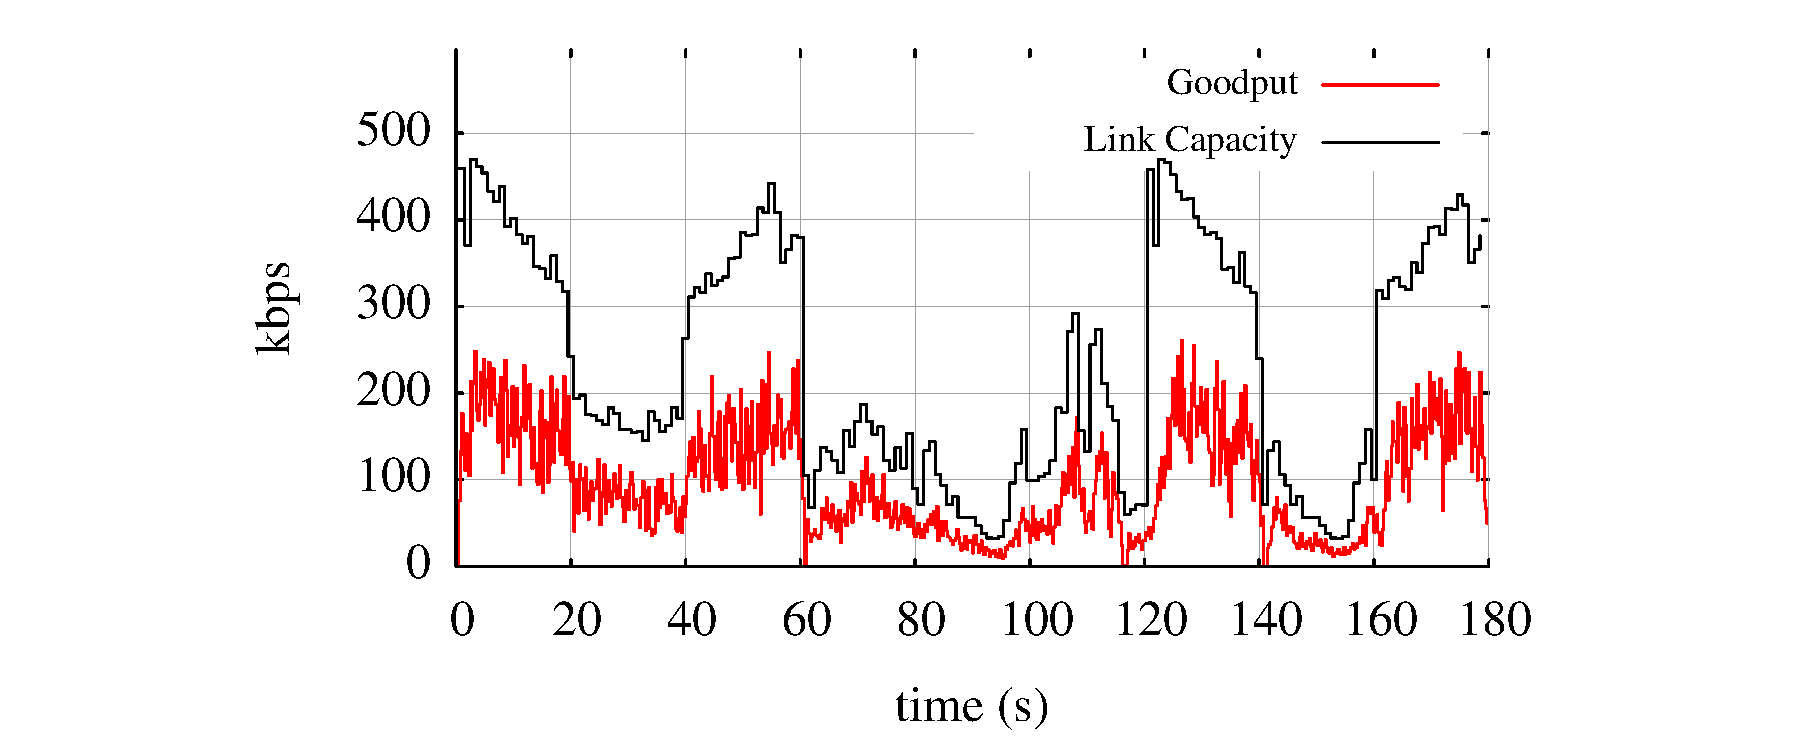
\includegraphics[width=0.5\textwidth, clip=true, trim=3cm 0 4.5cm 0]
      {chap8_graph_3g_tmmbr_a}
    }
    \subfloat{
      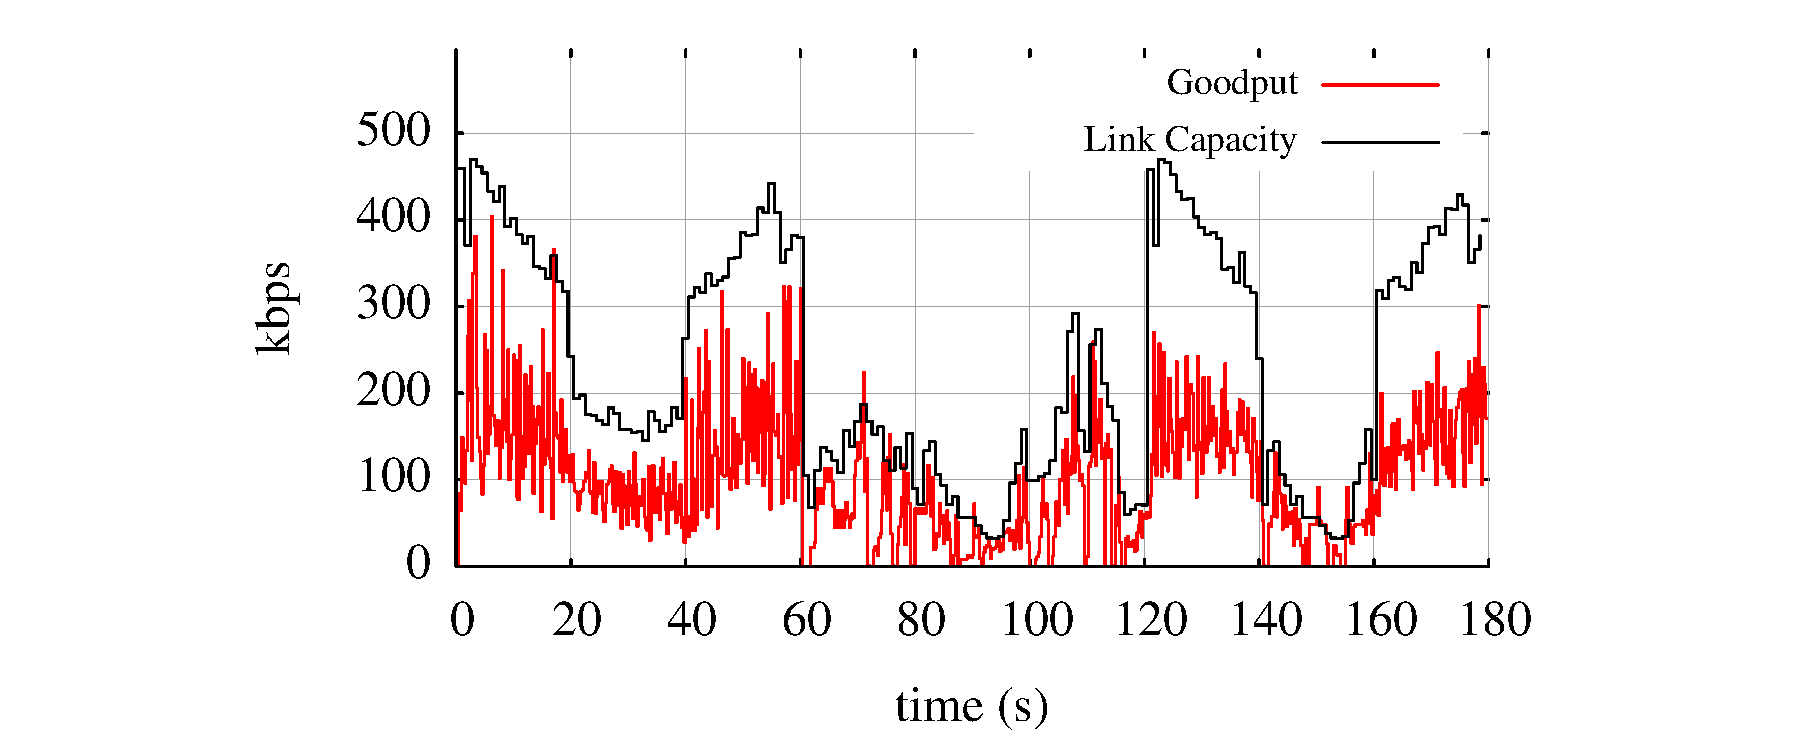
\includegraphics[width=0.5\textwidth, clip=true, trim=3cm 0 4.5cm 0]
      {chap8_graph_3g_tmmbr_b}
    }
  }
  \caption{Performance of C-NADU in a slow time-varying link and 3G network.}
  \label{fig:cnadu}
\end{figure}

\section{Out-of-path Source}

Congestion Maps